\documentclass[a4paper,12pt]{article}

\usepackage[utf8]{inputenc}
\usepackage[T1]{fontenc}
\usepackage{graphicx}
\usepackage{listings}
\usepackage{xcolor} 
\usepackage{booktabs}
\usepackage{geometry}

\geometry{a4paper, margin=1in}
\lstdefinelanguage{Cypher}{
  keywords={TOSTRING, MATCH, RETURN, CREATE, DELETE, WHERE, SET, MERGE, LIMIT, DISTINCT, COLLECT, COALESCE, COUNT, END, WHEN, ELSE, IS NOT NULL, THEN, OPTIONAL},
  sensitive=true,
  comment=[l]{//},
  morecomment=[s]{/*}{*/},
  morestring=[b]",
  morestring=[b]'
}
% Ustawienie wyglądu tytułu
\title{\vspace{2cm} \textbf{\Huge Kryminalne zagadki} \\[1cm] \large Uniwersytet Gdański \\ Grafowe Bazy Danych \vspace{2cm}}

% Autorzy i data
\author{\textsc{Michał Redkwa, Maciej Marzec}}
\date{12.01.2025}

\begin{document}

% Strona tytulowa
\maketitle

\newpage

\section{Wstęp}
\subsection{Założenia projektu}

W ramach projektu zaliczeniowego stworzyliśmy grafową bazę danych, której celem jest pokazanie, w jaki sposób za pomocą algorytmów i zapytań można zidentyfikować osobę odpowiedzialną za popełnienie przestępstwa. Na bazie zostały przeprowadzone zapytania, które pozwalają na wskazanie osób, które mogą być bezpośrednio związane z dowodami przestępstwa lub pełnić rolę potencjalnych świadków. Dzięki zastosowaniu zaawansowanych algorytmów, jesteśmy w stanie ocenić ich znaczenie w kontekście śledztwa oraz wytypować osoby o najmocniejszych powiązaniach z podejrzanymi.

\subsection{Opis wierzchołków oraz relacji pomiędzy nimi}

\begin{center}
    \textbf{\textit{Person}}
\end{center}

Wierzchołek \textbf{Person} reprezentuje osobę, posiada on właściwości: imię, nazwisko, wiek, długość oraz kolor włosów, kolor oczu, numer telefonu, numer konta bankowego oraz zawód jaki wykonuje. Jest on powiązany z następującymi wierzchołkami:

\begin{itemize}
    \item \textbf{Street} – relacja LIVES\_ON pomiędzy Person a Street.
    \item \textbf{Shop} – relacja BOUGHT\_AT lub VISITED pomiędzy Person a Shop. Relacja posiada dodatkowo właściwości, takie jak: typ wizyty, ilośc zakupów, ilośc wizyt.
    \item \textbf{Institution} – TODO ?? Zrobić powiązanie z bankiem jak ktoś ma tam konto?
\end{itemize}

\begin{center}
    \textbf{\textit{Street}}
\end{center}

Wierzchołek \textbf{Street} reprezentuje ulicę, zawiera takie własciowiści jak: nazwa, miasto, kod, typ. Ulice sa powiązane ze sobą za pomocą relacji CONNECTED\_TO.

\begin{center}
    \textbf{\textit{Institution}}
\end{center}

Wierzchołek \textbf{Institution} reprezentuje instytucję, jego własciowościami jest nazwa oraz jaki jest to typ instytucji. Wierzchołek ten powiązany jest z ulicami za pomocą relacji LOCATED\_AT.

\begin{center}
    \textbf{\textit{Shop}}
\end{center}

Wierzchołek \textbf{Shop} reprezentuje sklep. Posiada następujące własciwości: nazwa, typ oraz godziny otwarcia. Jest powiązany z ulicą za pomocą relacji LOCATED\_AT.

\begin{center}
    \textbf{\textit{Crime}}
\end{center}

Wierzchołek \textbf{Crime} reprezentuje zbrodnie. Posiada własciwości: typ przestępstwa, data, wyrok. Jest powiązany z daną ulicą, sklepem czy instytucją za pomocą relacji o nazwie COMMITTED\_AT.

\begin{center}
    \textbf{\textit{Evidence}}
\end{center}

Wierzchołek \textbf{Evidence} reprezentuje dowód, który posiada własciwości takie jak: typ, opis oraz date złożenia lub jego znalezienia. Jest powiązany z wierzchołkiem zbrodnia za pomocą relacji EVIDENCE\_IN.

\section{Zapytania Cypher}

\subsection{Proste rekomendacje - włamanie}

W ramach demonstracji przeszukiwania grafowej bazy danych naszym podejrzanym w przypadku włamania do sklepu będzie Paula Harris. Na początek wypiszmy wszystkie informacje jakie mamy o tej osobie.

\begin{center}
\begin{minipage}{0.8\linewidth}
\begin{lstlisting}[language=Cypher, basicstyle=\small, breaklines=true]
MATCH (p:Person {firstName: 'Paula', lastName: 'Harris'})-[r]->(related)
RETURN p, r, related
\end{lstlisting}
\end{minipage}
\end{center}

\begin{figure}[h!]
    \centering
    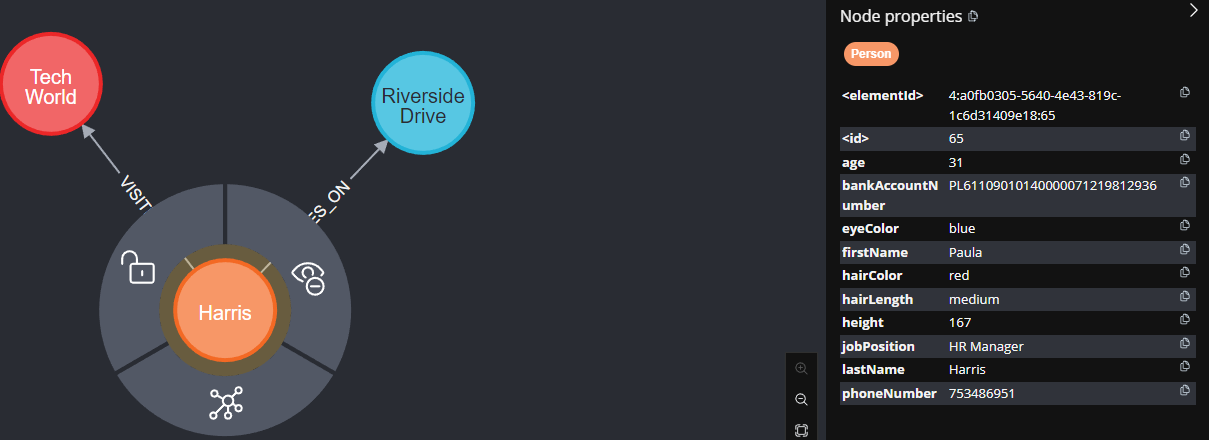
\includegraphics[width=0.7\textwidth]{paula_harris.png}
\end{figure}

Teraz prześledźmy wszystkie dowody związane ze sprawą włamania i spróbujmy na podstawie ich znaleźć osobę, która własnie jemu odpowiada.

\begin{center}
\begin{minipage}{0.8\linewidth}
\begin{lstlisting}[language=Cypher, basicstyle=\small, breaklines=true]
MATCH (n)-[r]->(m)
WHERE n.crimeType = 'Robbery' AND n.date = '2023-05-12' 
RETURN r, n, m;
\end{lstlisting}
\end{minipage}
\end{center}

\begin{figure}[h!]
    \centering
    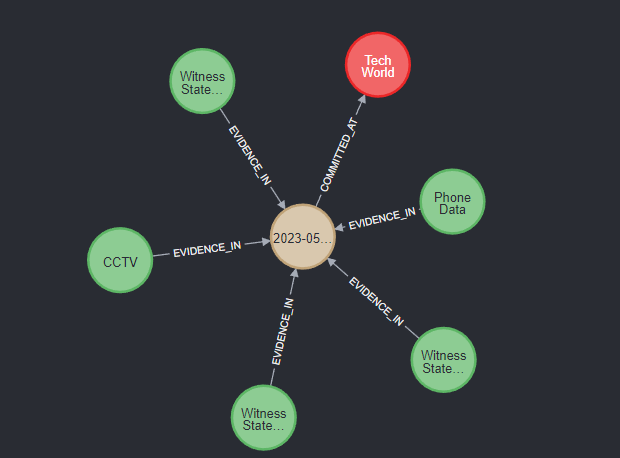
\includegraphics[width=0.7\textwidth]{robbery.png} 
\end{figure}

\newpage
Na podstawie zeznań świadków:

\begin{itemize}
    \item A witness reported seeing a person with medium-length red hair leaving the scene of the robbery at around 12:05 AM.
    \item A witness reported that the suspect had a height between 160 and 170 cm.
    \item A witness saw a person with red hair near the scene of the robbery at approximately 11:50 PM.
\end{itemize}

oraz nagrania z kamery, które wg opisu mówi nam: CCTV footage shows a person with medium-length red hair and blue eyes near the robbery location at 11:55 PM.
\newline
\newline Wyszukajmy osoby pasujące do tego rysopisu:

\begin{center}
\begin{minipage}{0.8\linewidth}
\begin{lstlisting}[language=Cypher, basicstyle=\small, breaklines=true]
MATCH (person:Person)
WHERE person.hairColor = 'red' AND person.height >= 160 AND person.height <= 170 AND person.eyeColor = 'blue'
RETURN person.firstName, person.lastName, person.height, person.hairColor, person.eyeColor
LIMIT 5;
\end{lstlisting}
\end{minipage}
\end{center}

\begin{table}[h!]
\centering
\begin{tabular}{|l|l|c|c|c|}
\hline
\textbf{First Name} & \textbf{Last Name} & \textbf{Height (cm)} & \textbf{Hair Color} & \textbf{Eye Color} \\ \hline
Daisy               & Anderson           & 160                 & red                 & blue               \\ \hline
Paula               & Harris             & 167                 & red                 & blue               \\ \hline
Wanda               & Holmes             & 170                 & red                 & blue               \\ \hline
Grace               & Reed               & 164                 & red                 & blue               \\ \hline
Maya                & Xavier             & 163                 & red                 & blue               \\ \hline
\end{tabular}
\caption{Tabela przedstawiająca dane osób z kolorem włosów "red" i kolorem oczu "blue".}
\label{tab:person_data_with_eyes}
\end{table}

Jak widać, mamy na naszej liście osobę, która popełniła to przestępstwo, jednak nie daje nam to ostatecznego potwierdzenia, że jest to osoba, która powinna zostać uznana za winną popełnionego przestępstwa. Został jeszcze jeden dowód z centrali telefonicznej w obrębie obszaru, gdzie popełniono przestępstwo.
\newline
\newline
"A phone with the number which ends on ...951 was found to have been frequently used near the crime scene, with activity under the alias "AngryVoice" reported around the time of the robbery."

\begin{center}
\begin{minipage}{0.8\linewidth}
\begin{lstlisting}[language=Cypher, basicstyle=\small, breaklines=true]
MATCH (person:Person)
WHERE toString(person.phoneNumber) ENDS WITH '951'
RETURN person.firstName, person.lastName, person.phoneNumber, person.hairColor, person.eyeColor
LIMIT 5;
\end{lstlisting}
\end{minipage}
\end{center}
\newpage
\begin{table}[h!]
\centering
\begin{tabular}{|l|l|l|l|l|}
\hline
\textbf{First Name} & \textbf{Last Name} & \textbf{Phone Number} & \textbf{Hair Color} & \textbf{Eye Color} \\ \hline
Paula              & Harris             & 753486951             & red                 & blue               \\ \hline
Henry              & Clark              & 852147951             & grey                & brown              \\ \hline
Emma               & Parker             & 852147951             & blonde              & green              \\ \hline
Brian              & Mills              & 456789951             & brown               & blue               \\ \hline
David              & Owens              & 753456951             & black               & brown              \\ \hline
\end{tabular}
\caption{Tabela przedstawiająca dane osobowe, numery telefonów oraz kolory włosów i oczu.}
\label{tab:person_data}
\end{table}

Jak widać, osoba którą podejrzewaliśmy znajduje się na tej liście - sprawa została rozwiązana.

\subsection{Proste rekomendacje - dodatkowe}

Zapytanie o osoby pasujące do opisu z monitoringu odnośnie zbrodni morderstwo:

\begin{center}
\begin{minipage}{0.8\linewidth}
\begin{lstlisting}[language=Cypher, basicstyle=\small, breaklines=true]
MATCH (person:Person)
WHERE person.hairColor = 'black' AND person.height >= 155 AND person.height <= 165
RETURN person.firstName, person.lastName, person.height, person.hairColor
LIMIT 5;
\end{lstlisting}
\end{minipage}
\end{center}

\begin{table}[h!]
\centering
\begin{tabular}{|l|l|c|l|}
\hline
\textbf{First Name} & \textbf{Last Name} & \textbf{Height (cm)} & \textbf{Hair Color} \\ \hline
Olive              & Hunt               & 164                  & black               \\ \hline
Bella              & Hughes             & 164                  & black               \\ \hline
Isabel             & Stevens            & 163                  & black               \\ \hline
Amy                & Lewis              & 160                  & black               \\ \hline
Isla               & Taylor             & 158                  & black               \\ \hline
\end{tabular}
\caption{Tabela przedstawiająca osoby z kolorem włosów "black" i wzrostem między 155 a 165 cm.}
\label{tab:black_hair_height}
\end{table}

Zapytanie o osoby, których inicjały mogą pasować do "IT", na znalezionym przedmiocie zbrodni:

\begin{center}
\begin{minipage}{0.8\linewidth}
\begin{lstlisting}[language=Cypher, basicstyle=\small, breaklines=true]
MATCH (person:Person)
WHERE substring(person.firstName, 0, 1) + substring(person.lastName, 0, 1) = 'IT'
RETURN person.firstName, person.lastName
LIMIT 5;
\end{lstlisting}
\end{minipage}
\end{center}

\begin{table}[h!]
\centering
\begin{tabular}{|l|l|}
\hline
\textbf{First Name} & \textbf{Last Name} \\ \hline
Ivy                & Taylor             \\ \hline
Isla               & Taylor             \\ \hline
Isabel             & Taylor             \\ \hline
Isaac              & Turner             \\ \hline
\end{tabular}
\caption{Tabela przedstawiająca osoby, których inicjały pasują do wyrytych na narzędziu zbrodni.}
\label{tab:names}
\end{table}
\newpage

Kolejna sprawa rozwiązana - naszym mordercą w tym przypadku jest Isla Taylor.

\subsection{Złożone zapytania}

\subsubsection{Grafowe przedstawienie powiązań do wykonywanych zapytań}

\begin{figure}[h!]
    \centering
    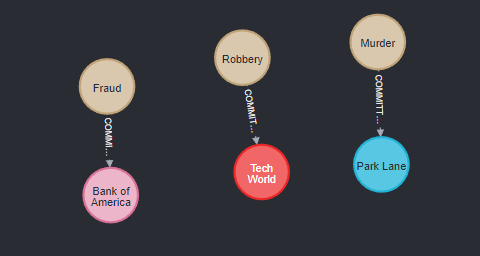
\includegraphics[width=0.7\textwidth]{commited_at.png}
    \caption{Graf przedstawiający połączenia dokonanych zbrodni z miejscem.}
    \label{fig:commited_at}
\end{figure}

\begin{figure}[h!]
    \centering
    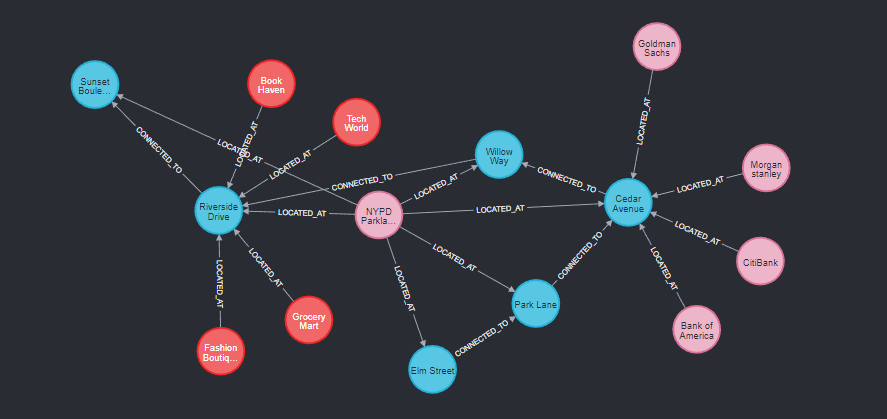
\includegraphics[width=0.7\textwidth]{located_at.png}
    \caption{Graf przedstawiający połączenia instytucji oraz sklepów z ulicami.}
    \label{fig:located_at}
\end{figure}

\subsubsection{Przykładowanie zapytania oraz wyniki}

1. Zapytanie, które ma na celu wskazanie potencjalnych świadków w odległości 2 od miejsca zbrodni włamanie.

\begin{center}
\begin{minipage}{0.8\linewidth}
\begin{lstlisting}[language=Cypher, basicstyle=\small, breaklines=true]
MATCH (crime:Crime)-[:COMMITTED_AT]->(location)-[:LOCATED_AT]->(street:Street),
      path = (street)-[:CONNECTED_TO*1..2]->(neighbor:Street)<-[:LIVES_ON]-(person:Person)
RETURN DISTINCT person.firstName, person.lastName, neighbor.name AS potentialWitnessLocation, street.name AS crimeLocation;
\end{lstlisting}
\end{minipage}
\end{center}

\begin{table}[h!]
\centering
\begin{tabular}{|c|l|l|l|l|}
\hline
\textbf{No.} & \textbf{First Name} & \textbf{Last Name} & \textbf{Potential Witness Location} & \textbf{Crime Location} \\ \hline
1            & Jack                & Lee                & Sunset Boulevard                   & Riverside Drive          \\ \hline
2            & Paul                & Evans              & Sunset Boulevard                   & Riverside Drive          \\ \hline
3            & Steve               & Morris             & Sunset Boulevard                   & Riverside Drive          \\ \hline
4            & Yara                & Collins            & Sunset Boulevard                   & Riverside Drive          \\ \hline
\multicolumn{5}{|c|}{\dots\dots\dots\dots} \\ \hline
33           & Victor              & King               & Sunset Boulevard                   & Riverside Drive          \\ \hline
\end{tabular}
\caption{Tabela przedstawiająca dane świadków i lokalizacje zdarzeń.}
\label{tab:witness_data}
\end{table}

2. Zapytanie, które zwróci w tabeli liczbę zbrodni w danej lokalizacji, jej ilość oraz typ.

\begin{center}
\begin{minipage}{0.8\linewidth}
\begin{lstlisting}[language=Cypher, basicstyle=\small, breaklines=true]
MATCH (crime:Crime)-[:COMMITTED_AT]->(location)
OPTIONAL MATCH (location)-[:LOCATED_AT]->(street:Street)
OPTIONAL MATCH (crime)-[:COMMITTED_AT]->(institution:Institution)
RETURN 
    COALESCE(street.name, location.name) AS StreetName, 
    COUNT(DISTINCT crime) AS CrimeCount, 
    COLLECT(DISTINCT CASE 
        WHEN institution IS NOT NULL THEN institution.institutionName 
        ELSE location.name 
    END) AS CrimeLocations,
    COLLECT(DISTINCT crime.crimeType) AS CrimeTypes;
\end{lstlisting}
\end{minipage}
\end{center}

\begin{table}[h!]
\centering
\begin{tabular}{|c|l|l|l|l|}
\hline
\textbf{No.} & \textbf{StreetName}     & \textbf{CrimeCount} & \textbf{CrimeLocations}     & \textbf{CrimeTypes} \\ \hline
1            & Riverside Drive         & 1                   &Tech World              & Robbery         \\ \hline
2            & Park Lane               & 1                   &Park Lane               & Murder          \\ \hline
3            & Cedar Avenue            & 1                   &Bank of America         & Fraud           \\ \hline
\end{tabular}
\caption{Tabela przedstawiająca dane dotyczące przestępstw, lokalizacji i typów przestępstw.}
\label{tab:crime_data}
\end{table}

\newpage
3. Podsumowanie wszystkich popełnionych zbrodni, zliczenie ilości dowodów i wymienienie ich typów.

\begin{center}
\begin{minipage}{0.8\linewidth}
\begin{lstlisting}[language=Cypher, basicstyle=\small, breaklines=true]
MATCH (crime:Crime)-[:COMMITTED_AT]->(location)
OPTIONAL MATCH (evidence:Evidence)-[:EVIDENCE_IN]->(crime)
RETURN 
    crime.crimeType AS CrimeType,
    COUNT(evidence) AS EvidenceCount,
    COLLECT(evidence.type) AS EvidenceTypes
ORDER BY EvidenceCount DESC;
\end{lstlisting}
\end{minipage}
\end{center}

\begin{table}[h!]
\centering
\begin{tabular}{|c|l|l|p{8cm}|}
\hline
\textbf{No.} & \textbf{CrimeType}     & \textbf{EvidenceCount} & \textbf{EvidenceTypes} \\ \hline
1            & Robbery & 5              & Witness Statement, Witness Statement, Phone Data, CCTV, Witness Statement \\ \hline
2            & Fraud & 4               & Fake Invoice, Bank Record, Witness Testimony, Email Record \\ \hline
3            & Murder & 2              & Security Footage, Murder Weapon \\ \hline
\end{tabular}
\caption{Tabela przedstawiająca dane dotyczące przestępstw oraz zebranych dowodów powiązanych z nimi}
\label{tab:crime_data}
\end{table}

4. Zebranie w tabelę ile ludzi żyje na danej ulicy, jakie są sklepy oraz instytucje.

\begin{center}
\begin{minipage}{0.8\linewidth}
\begin{lstlisting}[language=Cypher, basicstyle=\small, breaklines=true]
MATCH (s:Street)
OPTIONAL MATCH (i:Institution)-[:LOCATED_AT]->(s)
OPTIONAL MATCH (sh:Shop)-[:LOCATED_AT]->(s)
OPTIONAL MATCH (p:Person)-[:LIVES_ON]->(s)
WITH s, 
     collect(DISTINCT i.institutionName) AS Institutions, 
     collect(DISTINCT sh.name) AS Shops, 
     count(DISTINCT p) AS PeopleLiving
RETURN s.name AS Street, Institutions, Shops, PeopleLiving;
\end{lstlisting}
\end{minipage}
\end{center}

\begin{table}[h!]
\centering
\resizebox{\textwidth}{!}{
\begin{tabular}{|c|l|p{6cm}|p{5cm}|c|}
\hline
\textbf{No.} & \textbf{Street}          & \textbf{Institutions}                                                                                     & \textbf{Shops}                                                & \textbf{PeopleLiving} \\ \hline
1            & Elm Street               & NYPD Parklane, NYPD ElmStreet                                                                             & -                                                             & 41                   \\ \hline
2            & Park Lane                & NYPD Parklane                                                                                             & -                                                             & 33                   \\ \hline
3            & Cedar Avenue             & Bank of America, CitiBank, Goldman Sachs, Morgan Stanley, NYPD Parklane, NYPD CedaerAvaenue              & -                                                             & 36                   \\ \hline
4            & Willow Way               & NYPD Parklane, NYPD WillowWay                                                                             & -                                                             & 36                   \\ \hline
5            & Riverside Drive          & NYPD Parklane, NYPD Riverside                                                                             & Grocery Mart, Tech World, Fashion Boutique, Book Haven       & 38                   \\ \hline
6            & Sunset Boulevard         & NYPD Parklane, NYPD Sunset Boulevard, Hospital Sunset Boulevard                                           & -                                                             & 37                   \\ \hline
\end{tabular}
}
\caption{Tabela przedstawiająca dane dotyczące ulic, instytucji, sklepów oraz liczby mieszkańców.}
\label{tab:street_data}
\end{table}

5. Zebranie w tabelę ile osób wg. dowodów pasuje do popełnionej zbrodni (osobno).

\begin{center}
\begin{minipage}{0.8\linewidth}
\begin{lstlisting}[language=Cypher, basicstyle=\small, breaklines=true]
MATCH (p:Person)
WITH
    COUNT(CASE WHEN p.height >= 160 AND p.height <= 170 THEN 1 END) AS HeightBetween160And170,
    COUNT(CASE WHEN p.hairColor = 'red' THEN 1 END) AS RedHairColor,
    COUNT(CASE WHEN TOSTRING(p.phoneNumber) ENDS WITH '951' THEN 1 END) AS PhoneNumberEndsWith951,
    COUNT(CASE WHEN p.eyeColor = 'blue' THEN 1 END) AS BlueEyeColor
RETURN 
    HeightBetween160And170 AS `Height Between 160 and 170`, 
    RedHairColor AS `Red Hair Color`, 
    PhoneNumberEndsWith951 AS `Phone Number Ends With 951`,
    BlueEyeColor AS `Blue Eye Color`
\end{lstlisting}
\end{minipage}
\end{center}

\begin{table}[h!]
\centering
\begin{tabular}{|p{4cm}|p{4cm}|p{4cm}|p{4cm}|}
\hline
\textbf{Height Between 160 and 170} & \textbf{Red Hair Color} & \textbf{Phone Number Ends With 951} & \textbf{Blue Eye Color} \\
\hline
101 & 41 & 14 & 80 \\
\hline
\end{tabular}
\caption{Tabela przedstawiająca liczbę osób pasujących per dowód w sprawie włamania.}
\label{tab:criteria_counts}
\end{table}

\newpage

\section{Algorytmy}

\end{document}